\documentclass{cosas/tfg_domingo}
% \documentclass[numeros]{tfg_domingo}

\autor{Alejandro Martínez Floranes}
\titulo{Reescribir slatt en Python 3}
% Título corto para los encabezamientos de pagina:
\corto{} % En blanco si no es necesario recortarlo.
\ingles{Rewrite slatt in Python 3}
\fecha{julio de 2021}
% La normativa prescribe «cuatro o cinco palabras clave, en
% español y en inglés, para su indexación en el repositorio
% de TFG».
\palabras{reglas de asociación, hipergrafos, slatt, reescribir}%
  {association rules, hypergraph, slatt, rewrite}

\usepackage{lipsum} % Esto solo es relleno.
\usepackage{algorithm,algpseudocode}

\begin{document}

% Si alguna palabra se divide entre dos líneas en un punto
% indebido, podemos indicar aquí los puntos de corte
% aceptables (si los hay), p. ej,
% \hyphenation{ba-rro-co, frío, cria-do, su-per-ra-tón}
\hyphenation{Dijkstra new-speak}

\portada
\frontmatter
% \sucinto{A Sofía}
%\gracias{\input{cosas/agradecimientos.txt}}
\resumen{Las reglas de asociación son objetos matemáticos empleados de forma extensa en disciplinas como la minería de datos, aprendizaje automático y representación del conocimiento, entre otros campos.
Slatt es un proyecto de software libre desarrollado por José Luis Balcázar (Universidad Politécnica de Barcelona). Ofrece funcionalidades para el cálculo de reglas de asociación. Para ello, se apoya en implementaciones del algoritmo a priori para el cálculo de clausuras, el retículo de las clausuras y, entre otras
funcionalidades,devuelve las reglas representativas para cualquier elección de los parámetros de soporte y confianza.

En este proyecto, se ha mejorado este software utilizando como base las implementaciones disponibles en Slatt aplicadas a:

\begin{itemize}
    \item hipergrafos y algoritmos con aplicación a estos objetos;
    
    \item cálculo de clausuras y retículos (lattices);
\end{itemize}


Este trabajo ha requerido la búsqueda y análisis de algoritmos propuestos en la literatura científica sobre los puntos anteriores.
El lenguaje de desarrollo será Python3, encontrándose la implementación anterior en Python 2.7
%
% Conviene evitar aquí las llamadas a la bibliografía del
% trabajo, ya que el resumen tiene entidad independiente.
%

%% Aportamos nuestra perspectiva sobre la pertinencia de las
%% instrucciones {\tt goto}.


%%Pasar a tiempo presente
}{Association rules are mathematical objects used extensively in disciplines such as data mining, machine learning, and knowledge representation, among other fields.
Slatt is a free software project developed by José Luis Balcázar (Polytechnic University of Barcelona). It offers functionalities for the calculation of association rules. To do this, it relies on implementations of the a priori algorithm for the calculation of closures, the lattice of closures and, among others
functionalities, returns the representative rules for any choice of support and trust parameters.

In this project, this software has been improved using as a basis the implementations available in Slatt applied to:

\begin{itemize}
    \item hypergraphs and algorithms with application to these objects;
    
    \item calculation of closures and lattices (lattices);
\end{itemize}


This work has required the search and analysis of algorithms proposed in the scientific literature on the previous points.
The development language will be Python3, the previous implementation being in Python 2.7
}
\tableofcontents

\mainmatter
\chapter{Introducción}

Este proyecto se basa principalmente en reescribir \textbf{slatt} en Python 3 e incluir diferentes mejoras en el código para mejorar tanto su eficiencia en cuanto a rendimiento, como en reducción de lineas de código, y realizar una mejora en la legibilidad del propio código.

Slatt es un proyecto de software libre que ofrece funcionalidades para el cálculo de reglas de asociación. 

Las reglas de asociación son declaraciones 'if-then' que ayudan a mostrar la probabilidad de relaciones entre elementos de datos, dentro de grandes conjuntos de datos. Las reglas de asociación se miden a base a tres valores, \textit{el soporte, la confianza y el lift.}

\begin{itemize}
    \item El \textbf{soporte} es la frecuencia relativa de una regla sobre el total de las transacciones.
    \item La \textbf{confianza} mide que tan fiable es la suposición realizada por la regla de asociación.
    \item El \textbf{lift} es la confianza de la reglas dividido por el cociente del consecuente.
\end{itemize}


\begin{figure}[ht!] % [h!] fuerza que el elemento se sitúe
                    % en la posición señalada, en vez de al
                    % comienzo de una página.
\begin{center}
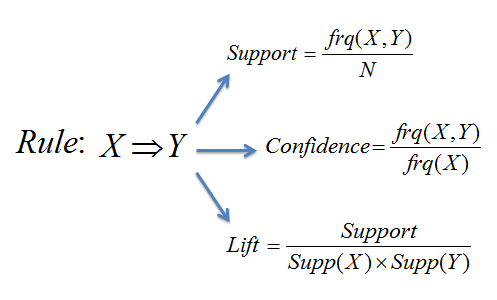
\includegraphics[width=.6\linewidth]{imagenes/AR_1.png}
\end{center}
\caption{Association Rules}
\label{fig_pro}
\end{figure}

% Utilice «citet» para integrar el nombre del autor en el
% texto. Para referencias aisladas, «citep».

\newpage

En dicho proyecto también se van a tratar elementos como los hipergrafos
y algoritmos con aplicación a estos.

Un hipergrafo H es una familia de subconjuntos (aristas) de un conjunto finito de vértices. Un hipergrafo es simple si ninguno de sus bordes está contenido en ningún otro de sus bordes. Decimos que un hipergrafo está saturado si cada subconjunto del conjunto de vértices está contenido en un borde o contiene un borde de el hipergrafo. \citep{Thomas}

Se toma como algoritmo principal \textit{The algorithm of Berge}, al cual se le añadirán diferentes mejoras analizadas y comprobadas en el paper desarrollado por \citep{JGAA-107} el cual implementa un algoritmo eficiente para la generación transversal de hipergrafos.


% Reproduce un fragmento de código.
\codigo[commandchars=\\\{\}]{codigo/berge.c}{Original}{7.5cm}
\hfill
\codigo{codigo/berjeMod.c}{Mejorado}{7.5cm}

% Añadiendo la opción «commandchars=\\\{\}», los caracteres
% \, { y } del archivo fuente se interpretan como código
% LaTeX y puede darse formato al código (manualmente). Hay
% que tener esto en cuenta cuando estos caracteres formen
% parte del código en sí.
%
% Sin esa opción, el fichero de reproduce tal cual.


\begin{center}
% Puede pasar parámetros al comando «VerbatimInput» del
% paquete «fancyvrb». Por ejemplo:
\codigo[numbers=none,frame=single]{codigo/berge.c}{}{11.5cm}
\end{center}

\newpage

Para la realización del proyecto se ha utilizado una metodología incremental, debido a que dicho proyecto esta dividido en diferentes partes, las cuales unas no tienen relación directa con otras, es por esto, que he decidió usar este tipo de metodología.

\begin{figure}[ht!] % [h!] fuerza que el elemento se sitúe
                    % en la posición señalada, en vez de al
                    % comienzo de una página.
\begin{center}
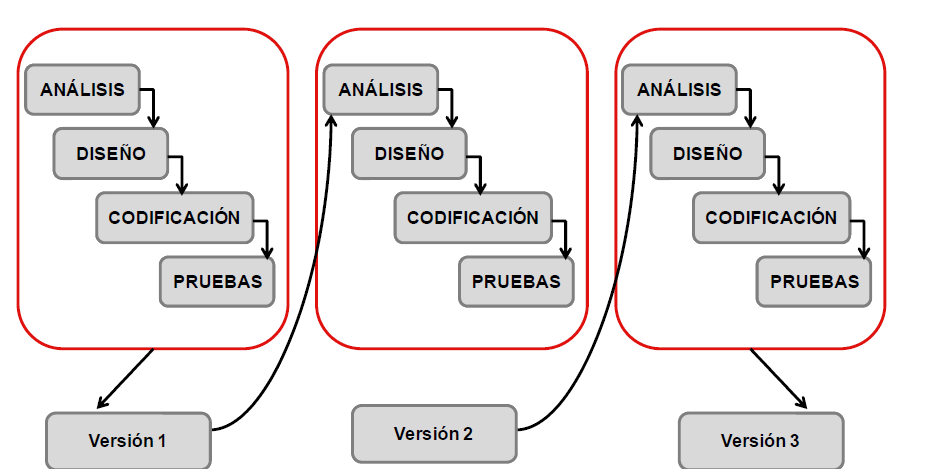
\includegraphics[width=.6\linewidth]{imagenes/Metodologia.png}
\end{center}
\caption{Metodologia iterativa incremental}
\label{fig_pro}
\end{figure}

\begin{table}[h]
\centering
\begin{tabular}{|l|l|}
\hline
Identificador & Descripción                                                                        \\ \hline
RF01          & La aplicación deberá tener la misma funcionalidad tanto en python2 como en python3 \\ \hline
RF02          & La mejora en python3 deberá ser mas eficiente que la de su anterior versión        \\ \hline
RF03          & La mejora en python3 deberá tener menos lineas de código que su anterior versión   \\ \hline
RF04          & La refactorización de los métodos no supondrá un cambio en los resultados          \\ \hline
\end{tabular}
\caption{Requisitos funcionales del proyecto}
\label{tab:my-table}
\end{table}


\begin{table}[h]
\centering
\begin{tabular}{|l|l|l|}
\hline
Identificador & Descripción                                                                           & Categoria \\ \hline
RNF01         & La aplicación deberá          & \\ \hline
RNF02         & La mejora en python3        &           \\ \hline
RNF03         & La mejora en python3    &           \\ \hline
RNF04         & La refactorización de l         &           \\ \hline
\end{tabular}
\caption{Requisitos no funcionales del proyecto}
\label{tab:my-table}
\end{table}



\chapter{\emph{Methodology Test}}

En esta sección se especifica como se realizan los test unitarios, para comprobar si las dos versiones del código mantienen la misma funcionalidad basándose en la salida de estos test.


\begin{verbatim}
##MAKEFILE##
##AUTHOR: ALEJANDRO MARTINEZ
##DATE: 26/03/2021

#Nombre_fich test python2 to python3
Nombre_fich : 

        python3 Python3/Nombre_fich.py > /home/usuario/Escritorio/TFG/tests/nombre_fich3.txt
        
        python2 Python2/Nombre_fich.py > /home/usuario/Escritorio/TFG/tests/nombre_fich2.txt
        
        diff /home/usuario/Escritorio/TFG/tests/nombre_fich3.txt
        
        /home/usuario/Escritorio/TFG/tests/nombre_fich3.txt >
        
        /home/usuario/Escritorio/TFG/tests/diff_nombre_fich.txt
\end{verbatim}

Utilizando este \textbf{makefile} se realiza una ejecución simultanea de ambas versiones, guardando dicha salida en un ficher .txt y a continuación, se hace un \textbf{diff} entre los dos archivos, en el caso en el que el \textbf{diff} devuelva un archivo vacio, sabremos que las dos versiones tienen la misma funcionalidad.

% Indique aquí el fichero .bib que contenga su bibliografía.
\bibliography{refs}

\end{document}
